\newpage
\section{R�alisation }
\label{sec:impl}

\subsection{L'ALU}
\label{sec:real1}

\paragraph{Composition}Notre ALU est donc compos� de :
\begin{itemize}
\item Un multiplexeur 
\item 8 op�rations
\end{itemize}

\begin{figure}[H]
	\centering
		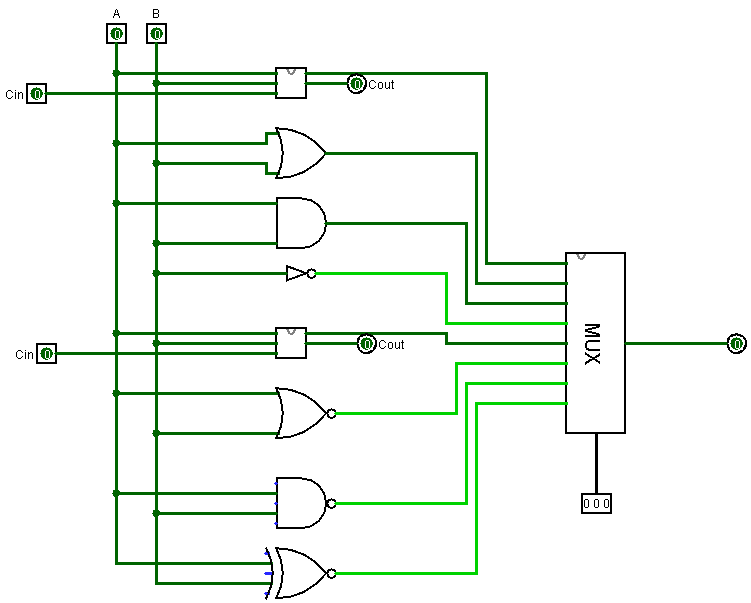
\includegraphics[width=15cm,height=10cm]{./img/ALU.png}
		\caption{Sch�ma complet de l'ALU}
	\label{fig:alu}
\end{figure}

\begin{figure}[H]
	\centering
		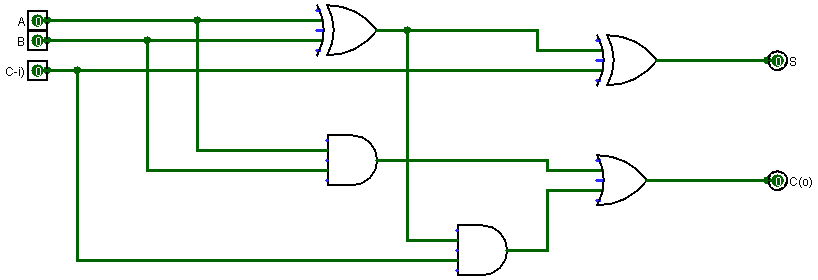
\includegraphics[width=12cm,height=8cm]{./img/fulladder.png}
		\caption{Sch�ma du FullAdder}
	\label{fig:fulladder}
\end{figure}

\begin{figure}[H]
	\centering
		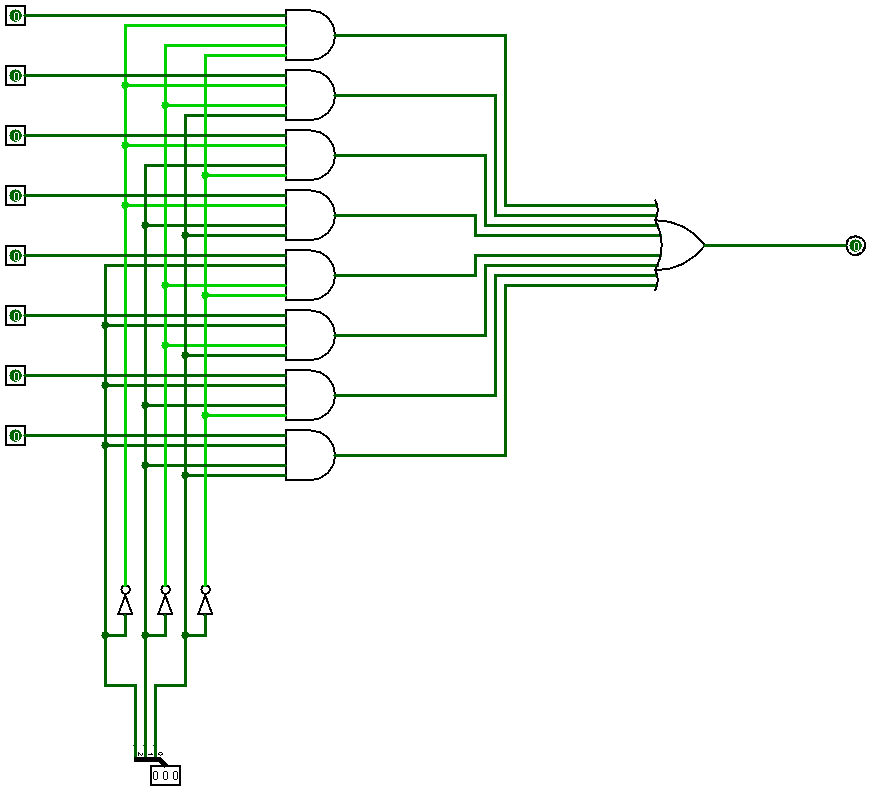
\includegraphics[width=15cm,height=10cm]{./img/MUX.png}
		\caption{Sch�ma du Multiplexeur}
	\label{fig:mux}
\end{figure}

\subsection{Le banc de registre}
\label{sec:real2}

\paragraph{} Notre banc de registre est ainsi :
\begin{itemize}
\item 4 registres 4 bits
\item un d�codeur
\item 2 s�lecteurs de registre (un pour le BUS X et l'autre pour le BUS Y)
\item Un s�lecteur de registre pour l'ecriture (sur 2 bits)
\item Un bit de validation pour l'�criture
\end{itemize}

\subsection{L'unit� d'adressage}
\label{sec:real3}

\paragraph{} 

\subsection{L'unit� de contr�le}
\label{sec:real4}

\paragraph{} Notre unit� de contr�le est compos�e d'un d�codeur et d'un registre d'instruction.

\subsection{Le CPU}
\label{sec:real5}

\paragraph{}Enfin pour concevoir le processeur il faut r�unir les diff�rentes parties vu ci-dessus.